% Einführung.tex
\chapter{Einführung} 
% TODO: Einführung 
\section{Unternehmensvorstellung} 
Eine Vorstellung des Unternehmens Unitedprint.

% Status: Erstprüfung 
\section{Der FreeDesign-Editor}
\label{Der FreeDesign-Editor}
\subsection{Funktionsbeschreibung}
Der, durch Unitedprint bereitgestellte, Webshop \emph{easyprint.com} bietet Kunden die Möglichkeit, Druckprodukt online zu gestaltet und im Anschluss zu bestellen. Für die Gestaltung der Produkte wurde die Webanwendung \emph{FreeDesign} entwickelt, welche beständig gepflegt und weiterentwickelt wird. Die Anwendung ist eine Single-Page-Application (SPA), was basieren auf Flanagan (\citeyear[S. 497]{Flanagan2006}) bedeutet, dass der Inhalt einer Webseite durch die Manipulation der HTML-Struktur per JavaScript aktualisiert wird und somit die Seite nicht komplett neu geladen werden muss. 

Mit Hilfe des FreeDesign-Editors kann eine große Vielzahl von Druckprodukten gestaltet werden, wobei das Portfolio verschiedenste Produktgruppen, wie Bürozubehör, Textilien oder Werbematerialien, abdeckt. Zur Gestaltung eines Designs bietet der Editor die Möglichkeit der Nutzung eigener Texte und Bilder sowie das Verwenden verschiedenster geometrischer Formen. Alle Elemente können umfangreich geometrisch und grafische bearbeitet werden. Um einen optimalen Gestaltungsprozess zu ermöglichen, kann die Produktdarstellung auch während der Gestaltung vergrößert, verschoben oder rotiert werden. Weiterhin stehen Hilfswerkzeuge wie Lineal oder Hilfslinien zur Verfügung. 

Die Nutzer haben auch die Möglichkeit Designs als Entwürfe zu speichern und zu einem späteren Zeitpunkt zu öffnen.

\begin{figure}[H]
    \centering
    \efbox{\includegraphics[width=.98\textwidth]{chapter/freedesign/Screenshot-FreeDesign.png}}
    \caption{Ein Bildschirmfoto des FreeDesign-Editor}
    \label{fig:Der FreeDesign-Editor}
\end{figure}

\subsection{Designvorlagen}
\label{sect:Designvorlagen}
Um das Gestalteten der Produkte zu erleichtern, werden eine Vielzahl von Designvorlagen zur weiteren Gestaltung im Webshop angeboten. 
Aktuell (März 2021) werden die Designvorlagen in deutsch und englisch angeboten. Jedoch sollen in Zukunft die Designvorlagen auch in den restlichen Sprachen, in denen \emph{easyprint.com} zur Verfügung steht angeboten werden. 
Jede Designvorlage steht in verschiedenen Farbvarianten, welche als Farbschemen bezeichnet werden, zur Verfügung. Abbildung \ref{fig:Designuebersichtseite} zeigt den Aufbau einer Übersichtseite für die Designvorlagen, über welche der Nutzer eine Vorlage zur weiteren Bearbeitung im FreeDesign-Editor auswählen kann. Im Linken Menü kann, über das Untermenü mit den Farbkreisen, ein Farbschema für alle Designvorlagen der Seite gewählt werden. Es ist jedoch auch Möglich, innerhalb des Vorschaubildes das Farbschema für ein einzelnes Design zu wechseln.
Die Varianten einer Designvorlage werden im folgenden als Designderivate bezeichnet. 
Durch die Kombination aus Sprachen und Farbschemen werden aktuell je Design 20 Farb/Sprach-Derivate angeboten.
\begin{center}
    \efbox{Farb/Sprach-Derivate=Fabderivate*Sprachderivate}
\end{center}

\begin{figure}[H]
    \centering
    \efbox{\includegraphics[width=.98\textwidth]{chapter/freedesign/Screenshot-Designseite.png}}
    \caption{Ein Bildschirmfoto der Übersichtseite für Designvorlagen}
    \label{fig:Designuebersichtseite}
\end{figure}

Unitedprint betreibt auch das Webportal \emph{design.easyprint.com}, in welchem Designvorlagen, mit Hilfe des FreeDesign-Editors, gestaltet und zur Veröffentliche eingereicht werden können. Wird eine Designvorlage durch die Innovationsabteilung des Unternehmens angenommen, durchläuft es einen Integrationsprozess für die Bereitstellung im Webshop. Sie Person, die die Vorlage gestaltet hat, erhält ein Honorar für die erfolgreiche Einreichung.




% \subsubsection{Externe Schnittstellen}
Der FreeDesign-Editor kommuniziert über folgende vier Schnittstellen:
\begin{itemize}
	\item Über eine grafische Oberfläche wird der Editor vom Nutzer bedient und die Anwendung reagiert sowohl auf Mauseingaben als auch auf Tastatureingaben. 
	\item Zur Kommunikation mit Unitedprint-Backend wird eine REST-API genutzt. 
	\item Der Editor wird mit einer Reihen von URL-Parametern aufgerufen, die steuern, welche Produkt-Konfiguration von der Anwendung geladen wird. Über die URL-Parameter kann auch das Laden von Designvorlagen oder Kundendesign gesteuert, sowie weiter Funktionalitäten des Editors aktiviert werden. 
	Innerhalb des Editor besteht auch die Möglichkeit das Produkt zu ändern, worauf hin die URL sich aktualisiert.
	\item Ein Browser-Cookie wird vorwiegend zur Nutzer-Authentifizierung genutzt. 
\end{itemize}

Browser bieten die Möglichkeiten Daten in einem Local-Storage-Object oder einem Session-Storage-Object Daten zu speichern. \autocite[vgl.][]{Mozilla:Storage}
Die werden jedoch aktuell von der Anwendung nicht genutzt. 

% TODO: Es fehlt das Clipboard

\begin{figure}[H]
    \centering
    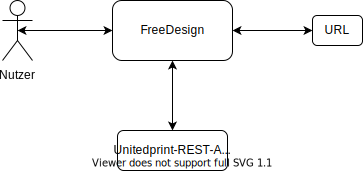
\includegraphics{diagrams/Ist-Architektur/Freedesign_Interaktion.pdf}
     \caption{Externe Schnittstellen}
     \label{fig:Externe_Schnittstellen}
  \end{figure}
  

\section{Problemstellung}
Als Anfang 2018 die Entwicklung der aktuellen FreeDesign-Anwendung begonnen wurde, hatte das Team nur wenig Erfahrung im Entwickeln von ReactJS-Anwendungen. Des Weiteren wurde die Anwendung unter einem hohen zeitlichen Druck entwickelt.
Dadurch sind eine Reihe von technischen Schulden entstanden. Eine der Hauptschulden ist eine fehlende Definition der Quelltext-Architektur. Durch die Verwendung von ReactJS und Redux wird zwar bereits eine gewisse Architektur vorgeben, diese bezieht sie jedoch auf die Strukturierung der grafischen Oberfläche. Für die Domain-Logik wurde jedoch keine spezifische Architektur festgelegt, was die Pflege und Weiterentwicklung der Anwendung, erschweren kann.
Die aktuelle Architektur weist derzeit folgende offensichtliche Schwächen auf:
\begin{itemize}
  \item Die Architektur ist nicht dokumentiert.
  \item Der Quelltext für die grafische Oberfläche und für die Domain-Logik sind mitunter viel
  zu eng gekoppelt, was den Austausch und die Aktualisierung von JavaScript-
  Bibliotheken erschwert.
  \item Durch die zuvor genannte enge Kopplung ist es für einige Teile des Quelltextes
  schwer Unit-Tests zu erstellen bzw. zu pflegen.
  \item Einige Teile des Quelltextes weisen Anzeichen von Anti-Patterns auf.
\end{itemize}
Da die Anwendung einer permanenten Weiterentwicklung unterliegt, ist es wichtig die Software in eine geeignetere Architektur zur überführen. Weiterhin entwickelt sich die Webtechnologie mit großer Geschwindigkeit weiter. An dieser Stelle ist eine Architektur notwendig, die eine effiziente Pflege ermöglicht.

\section{Ziel der Diplomarbeit}
Das Ziel der Diplomarbeit ist die Ausarbeitung eines Vorgehens zur Überführung einer Ist-Architektur einer, in TypeScript implementierten, ReactJS-Anwendung in eine Soll-Architektur. Um eine hohe Akzeptanz einer solcher Maßnahme zu erreichen, ist eine Rahmenbedingung, dass die Überführung schrittweise geschieht und die Weiterentwicklungsarbeit der ReactJS-Anwendung begleitet.
